% Chapter 4
\label{Capítulo4}
\chapter{Implementação}
\begin{center}
    \textit{``Do or do not. There is no try.''}
     
     Master Yoda
\end{center}
Neste capítulo aborda-se com mais pormenor os aspectos mais técnicos do \acrshort{lare}, tendo como base a arquitectura apresentada na Figura \ref{fig:arquitecturalore}.

O desenvolvimento começou pela implementação e desenvolvimento do servidor \textit{Flask} e página \textit{web}. O primeiro circuito a ser testado e integrado foi a Lei de Ohm. O projecto foi evoluindo com a adição dos restantes circuitos que compõem o \acrshort{lare}.

O \acrshort{ide} utilizado no desenvolvimento do \textit{software} foi o \textit{Visual Studio Code}\footnote{\url{https://code.visualstudio.com/}} e o projecto está alojado no \textit{GitHub}. O sistema operativo instalado no RaspberryPI 5 foi uma versão ligeiramente modificada do \textit{Arch Linux ARM}.

\section{Servidor Flask}
\textbf{Não sei se ainad vai ficar desta forma}

Hoje em dia vive-se (n)uma Era em que toda a informação está disponível na ``ponta dos dedos'' e à distância de um \textit{click}. A pesquisa, desenvolvimento e teste dos assuntos mais técnicos revelou-se longa e muitas vezes extenuante. Os recursos são (quase) incomensuráveis e o grande desafio é tentar perceber a dicotomia certo/errado. Recorreu-se à Inteligência Artificial, documentação técnica \textit{online}, fóruns de discussão, ajuda pessoal, tutoriais \textit{online} e vídeos no YouTube. 

A base para a implementação do \textit{Flask} e \underline{\textbf{toda a informação descrita neste}} \underline{\textbf{capítulo}} teve como base a documentação técnica disponível no \textit{site} do \href{https://flask.palletsprojects.com/en/3.0.x/}{\textit{Flask}} e complementada com alguns tutoriais do \textit{Youtube}, como por exemplo: \href{https://www.youtube.com/watch?v=dam0GPOAvVI}{\textit{link}} ou \href{https://www.youtube.com/watch?v=bB6Yyh7nUl4}{\textit{link}} .

\subsection{Estrutura base}
O fluxograma apresentado na Figura \ref{fig:funcflask} apresenta o funcionamento geral do servidor \textit{Flask}.

\begin{figure}[hbtp]
    \centering
    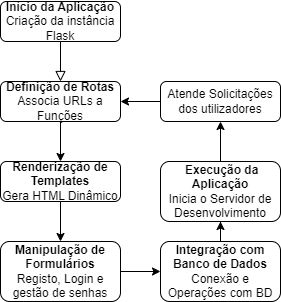
\includegraphics[width=0.7\textwidth]{figures/fluxograma_flask.drawio.png}
    \caption{Funcionamento geral \textit{Flask}}
    \label{fig:funcflask}
\end{figure}

A estrutura de directórios do \textit{Flask} tem uma base pré-definida que não é necessariamente rígida e pode ser adaptada consoante os requisitos do projecto \cite{Flask}. No caso do \acrshort{lare} a estrutura ficou organizada da forma como se mostra na Figura \ref{fig:estruturapastas}

\begin{figure}[hbtp]
    \centering
    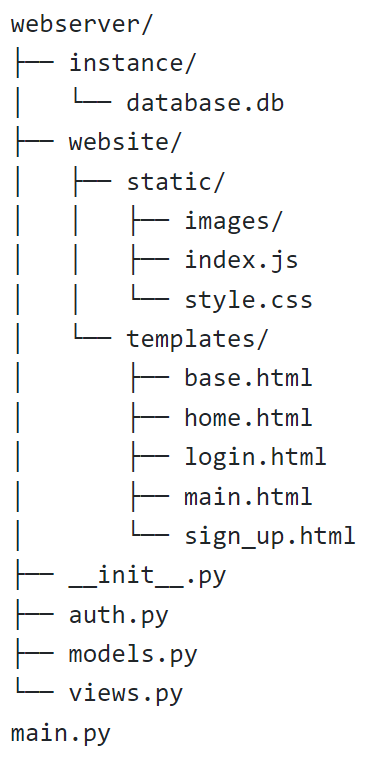
\includegraphics[width=0.3\textwidth]{figures/tree_flask.png}
    \caption{Estrutura de directórios - \textit{Flask} \textbf{ main.html está a mais}}
    \label{fig:estruturapastas}
\end{figure}

A raiz do projecto é o directório ``\textit{webserver}'' e nele estão contidos o ficheiro principal, assim como outros directórios e ficheiros de configuração essenciais:
\begin{itemize}
    \item \textit{main.py}: O ficheiro principal do aplicativo que inicializa e configura o \textit{Flask};
    \item \textit{requirements.txt}: Uma lista de dependências do projeto que podem ser instaladas usando \gls{pip};
    \item \textit{static/}: Este diretório contém os ficheiros estáticos como \acrshort{css}, \textit{JavaScript} e as imagens usadas em toda a aplicação;
    \item \textit{templates/}: Contém os modelos \acrshort{html} usado para renderizar as visualizações;
    \item \textit{instance/}: Diretório para armazenar ficheiros de configuração ou ficheiros que mudam em tempo de execução, específicos da cada instância, por exemplo, ficheiros da base de dados.
\end{itemize}

Dentro da raiz, criou-se o directório \textit{website} onde se incluiu os ficheiros respeitantes ao funcionamento do \textit{site}. Nele constam os já descritos \textit{templates}, \textit{static} e ainda os seguintes ficheiros:

\begin{itemize}
    \item \textit{\_\_init\_\_.py}: Inicializa o \textit{Flask} e define as configurações. Este ficheiro dentro da directoria \textit{website} faz com que esta seja tratada como um pacote \textit{Python}. Isto quer dizer que a directoria pode ser importada e tudo o que estiver dentro é executado automaticamente;
    \item \textit{views.py}: Contém as funções de visualização para o tratamento de pedidos \acrfull{http};
    \item \textit{models.py}: Define os modelos de dados para a aplicação;
    \item \textit{auth.py}: Este ficheiro é responsável por lidar com a autenticação e autorização de utilizadores, pode incluir funções e rotas que permitem aos utilizadores registarem-se, fazer \textit{login} e fazer \textit{logout}.
\end{itemize}

\subsection{Rotas}
As aplicações \textit{Web} modernas utilizam \acrshort{url}s amigáveis para ajudar os utilizadores a memorizar e utilizar o nome para voltar a visitar diretamente uma página.

No \textit{Flask} utiliza-se o decorador \textit{\textbf{route()}} para associar uma função a um \acrshort{url}, tal como pode ser visto na Listagem \ref{lst:decoradorroute}.

\begin{minipage}{0.9\linewidth}
\begin{lstlisting}[language=Python, caption=Decorador \textit{route()} - \textit{views.py}, label=lst:decoradorroute]
@views.route("/ohm", methods=['GET', 'POST'])
@login_required
def pagina_seguinte():
    return render_template("ohm.html", user=current_user)
\end{lstlisting}
\end{minipage}

O decorador \textit{\textbf{route}} define uma rota para a \acrshort{url} \textit{ohm}. Esta rota aceita pedidos \acrshort{http} de métodos \textit{GET} e \textit{POST}.

O decorador \textit{\textbf{login}} garante que o utilizador tem de estar autenticado para aceder a esta rota. Se o utilizador não estiver autenticado, será redirecionado para a página de \textit{login}.

A função pagina\_seguinte() é executada assim que a respectiva rota for acedida.

A última linha renderiza o \textit{template} \textit{\textbf{home.html}} e passa o objecto \textit{current\_user} para o \textit{template}.

Para construir um \acrshort{url} para uma função específica, usa-se a função \textit{\textbf{url\_for()}}. Esta função aceita o nome da função como seu primeiro argumento e qualquer número de argumentos de palavras-chave, cada um correspondendo a uma parte variável da regra de \acrshort{url}, tal como pode ser visto na Listagem \ref{lst:urlfor}

\begin{minipage}{0.9\linewidth}
\begin{lstlisting}[language=Python, caption=Contrução de \textit{url}s - \textit{auth.py}, label=lst:urlfor]
(...)
if user:
    if check_password_hash(user.password, password):
        flash('Logged in successfully!', category='success')
        login_user(user, remember=True)
        return redirect(url_for('views.home'))
(...)
\end{lstlisting}
\end{minipage}

Isto quer dizer que o \textit{Flask} gera a \acrshort{url} correspondente à função \textit{\textbf{home()}} definida no ficheiro \textit{\textbf{views.py}} dentro da \textit{Blueprint} \textit{views}. Quando usada dentro de \textit{\textbf{redirect}}, redireciona o utilizador para essa \acrshort{url}.

\subsection{Blueprints}
O \textit{Flask} usa um conceito de \textit{blueprints} para criar componentes de aplicações e suportar padrões comuns dentro de uma aplicação ou entre aplicações. As \textit{blueprints} podem simplificar muito o funcionamento de grandes aplicações e fornecer um meio central para que as extensões do \textit{Flask} registem operações em aplicações. As \textit{blueprints} permitem organizar a aplicação em partes menores e de mais fácil gestão. O conceito básico das \textit{blueprints} é que registam as operações a executar quando são integrados numa aplicação. O \textit{Flask} associa funções de vista (\textit{views}) a \textit{blueprints} quando processa pedidos e gera \acrshort{url} entre diferentes pontos de acesso.

Nas Listagens \ref{lst:blueprintviews} e \ref{lst:blueprintauth} podem ver-se as duas \textit{blueprints} definidas no caso da implementação do \acrshort{lare}.
\begin{center}
\begin{minipage}{0.7\linewidth}
\begin{lstlisting}[language=Python, caption=\textit{Blueprint views} - \textit{views.py}, label=lst:blueprintviews]
views = Blueprint('views', __name__)
\end{lstlisting}
\end{minipage}
\end{center}

\begin{center}
\begin{minipage}{0.7\linewidth}
\begin{lstlisting}[language=Python, caption=\textit{Blueprint auth} - \textit{auth.py}, label=lst:blueprintauth]
auth = Blueprint('auth', __name__)
\end{lstlisting}
\end{minipage}
\end{center}

Ambas as \textit{blueprints} são registadas no ficheiro \textit{\_\_init\_\_.py}, como se pode verificar na Listagem \ref{lst:initreg}

\begin{center}
\begin{minipage}{0.7\linewidth}
\begin{lstlisting}[language=Python, caption=Registo das \textit{blueprints} - \textit{\_\_init\_\_.py}, label=lst:initreg]
app.register_blueprint(views, url_prefix='/')
app.register_blueprint(auth, url_prefix='/')
\end{lstlisting}
\end{minipage}
\end{center}

Isto quer dizer que ao registar a \textit{blueprint} com o prefixo ``/'', os \acrshort{url}s serão acessíveis através da raiz da aplicação.

\subsection{Pedidos}
A capacidade de uma aplicação \textit{web} em responder a solicitações de dados do cliente é um requisito essencial. No \textit{Flask} esta informação é fornecida pelo objeto global \textit{\textbf{request}}. Este objeto contém todos os detalhes da solicitação, como os métodos \acrshort{http} usados (\textit{GET}, \textit{POST}, etc.), os \textit{headers} os \textit{cookies} ou o corpo da requisição.

O método de requisição pode ser determinado através do atributo \textit{\textbf{method}}. Para aceder aos dados de um formulário (transmitidos numa requisição \textit{POST} ou \textit{PUT}), utiliza-se o atributo \textit{\textbf{form}}, tal como pode ser visto na Listagem \ref{lst:atributorequest}.

\begin{minipage}{0.9\linewidth}
\begin{lstlisting}[language=Python, caption=Exemplo atributo \textit{\textbf{request} - \textit{auth.py}}, label=lst:atributorequest]
@auth.route('/login', methods=['GET', 'POST'])
def login():
    if request.method == 'POST':
        email = request.form.get('email')
        password = request.form.get('password')

        user = User.query.filter_by(email=email).first()
        if user:
            if check_password_hash(user.password, password):
                flash('Logged in successfully!', category='success')
                login_user(user, remember=True)
                return redirect(url_for('views.home'))
            else:
                flash('Incorrect password, try again.', category='error')
        else:
            flash('Email does not exist.', category='error')

    return render_template("login.html", user=current_user)
\end{lstlisting}
\end{minipage}

Quando se adiciona um ponto de interrogação (?) seguido de pares chave-valor (key=value) no final de um \acrshort{url}, está a enviar-se dados adicionais ao servidor, esses dados são chamados de \textbf{parâmetros do \acrshort{url}}, como se pode ver na Listagem \ref{lst:paramurl}.

\begin{minipage}{0.9\linewidth}
\begin{lstlisting}[language=Python, caption=Exemplo atributo \textit{\textbf{args} - \textit{views.py}}, label=lst:argrequest]
@views.route('/config_VirtualBench', methods=['GET', 'POST'])
@login_required
def config_VirtualBench():
    try:
        Vcc = request.args.get('Vcc', 0, int)
        Resistance = request.args.get('R', 0, int)
        (...)
    except Exception as e:
        print(e)
        return jsonify({'measurement_result': 'ERROR'})
    finally:
        return jsonify({'measurement_result': measurement_result})
\end{lstlisting}
\end{minipage}

\begin{minipage}{0.9\linewidth}
\begin{lstlisting}[language=Html, caption=Exemplo argumentos passados ao servidor - ohm.html, label=lst:paramurl]
const url = `/config_VirtualBench?parameter=${parameter}&Vcc=${Vcc}&R=${Resistance}`;
\end{lstlisting}
\end{minipage}

No entanto, a criação e renderização das páginas \acrshort{html} é feita automaticamente através dos modelos \textit{Jinja2}\footnote{A documentação pode ser consultada em \href{https://jinja.palletsprojects.com/en/3.1.x/templates/}{\textit{Jinja}}}. Os modelos podem ser usados para gerar qualquer tipo de ficheiro de texto, sendo que para aplicações \textit{web} serão, principalmente, páginas \acrshort{html}.

Na Listagem \ref{lst:htmljinja2} pode ver-se um exemplo da combinação entre código \acrshort{html} e sintaxe \textit{Jinja2}.

\begin{minipage}{0.9\linewidth}
\begin{lstlisting}[language=Html, caption=Exemplo sintaxe \textit{Jinja2} - base.html, label=lst:htmljinja2]
<title>Home</title>
  </head>
  <body>
    <nav class="navbar navbar-expand-lg navbar-dark bg-dark">
      <button
        class="navbar-toggler"
        type="button"
        data-toggle="collapse"
        data-target="#navbar"
      >
        <span class="navbar-toggler-icon"></span>
      </button>
      <div class="collapse navbar-collapse" id="navbar">
        <div class="navbar-nav">
          
          <a class="nav-item nav-link" id="home" href="/">Home</a>
          <a class="nav-item nav-link" id="logout" href="/logout">Logout</a>
          
          <a class="nav-item nav-link" id="login" href="/login">Login</a>
          <a class="nav-item nav-link" id="signUp" href="/sign-up">Sign Up</a>
          
        </div>
      </div>\end{lstlisting}
\end{minipage}

No código \acrshort{html}, encontram-se secções entre chavetas {} com palavras-chave especiais como por exemplo {\% block \%} e {\% endblock \%}. Estes são blocos de modelo \textit{Jinja2} que definem áreas de conteúdo dinâmico que podem ser preenchidas com lógica ou dados em \textit{Python}.

Para renderizar um modelo, o método utilizado foi \textit{\textbf{render\_template()}}, como pode ser visto na Listagem \ref{lst:atributorequest}, linha 18. O \textit{Flask} procurará por modelos na pasta \textit{templates}, como pode ser visto na Figura \ref{fig:estruturapastas}.

Na página oficial do \textit{Flask} é recomendado que se aceda aos parâmetros do \acrshort{url} com \textit{\textbf{get}} ou capturando o \textit{\textbf{KeyError}}, uma vez que os utilizadores podem alterar o \acrshort{url} e, nesse caso, apresentar uma página \textit{400 bad request} não é de fácil interpretação.

\subsection{Base de dados}
A aplicação desenvolvida usa uma base de dados e autenticação de utilizador, a ligação com a base de dados é aberta no início do pedido e é obtida a informação do utilizador. No final do pedido, a ligação com a base de dados é fechada.

No contexto da documentação do \textit{Flask} e implementação de uma base de dados, são apresentados duas alternativas: \textit{SQLite 3} e \textit{ SQLAlchemy}. Tal como referenciado/aconselhado na documentação, usou-se a extensão \textit{Flask-SQLAlchemy}, como apresentado na Listagem \ref{lst:basedados}

\textbf{Nota para minha referência: Falar de instalar o pacote SQLAlchemy?}

\begin{minipage}{0.9\linewidth}
\begin{lstlisting}[language=Python, caption=Exemplo uso \textit{ SQLAlchemy} - \textit{\_\_init.py\_\_}, label=lst:basedados]

from flask_sqlalchemy import SQLAlchemy

db = SQLAlchemy()
DB_NAME = "database.db"

def create_app():
    app = Flask(__name__)
    app.config['SECRET_KEY'] = 'hjshjhdjah kjshkjdhjs'
    app.config['SQLALCHEMY_DATABASE_URI'] = f'sqlite:///{DB_NAME}'
    db.init_app(app)
(...)
\end{lstlisting}
\end{minipage}

\subsection{Autenticação}
A segurança da aplicação é feita com recurso à página de \textit{login} e \textit{logout}, para isso foi instalada a extensão \textit{flask-login}, tal como é apresentado na Listagem \ref{lst:exemplologin}

\begin{minipage}{0.9\linewidth}
\begin{lstlisting}[language=Python, caption=Exemplo autenticação \textit{login}, label=lst:exemplologin]
@auth.route('/login', methods=['GET', 'POST'])
def login():
    if request.method == 'POST':
        email = request.form.get('email')
        password = request.form.get('password')

        user = User.query.filter_by(email=email).first()
        if user:
            if check_password_hash(user.password, password):
                flash('Logged in successfully!', category='success')
                login_user(user, remember=True)
                return redirect(url_for('views.home'))
            else:
                flash('Incorrect password, try again.', category='error')
        else:
            flash('Email does not exist.', category='error')
    return render_template("login.html", user=current_user) 
\end{lstlisting}
\end{minipage}

\section{pyVirtualBench}
Antes de se avançar para uma explicação mais pormenorizada das experiências, importa enquadrar o \textit{pyVirtualBench} no contexto do \textit{software}. Já foi referido na Secção \ref{sec:solucaoproposta} que o \textit{pyVirtualBench} é um \textit{wrapper} que permite controlar o \acrshort{virtualbench} a partir de uma aplicação \textit{Python}. Viu-se também que este \textit{wrapper} não é compatível com \textit{Linux} e não é suportado oficialmente pela \acrshort{ni}. Por isso, toda a programação, controlo e configuração do \acrshort{virtualbench} foi realizada com base neste \textit{wrapper} que pode ser transferido ou consultado no \href{https://github.com/armstrap/armstrap-pyvirtualbench/tree/master}{GitHub}.

Além de instalar a biblioteca, os autores disponibilizam uma série de exemplos, sendo que, aqueles que mais se enquadram nos objectivos deste projecto são:
\begin{itemize}
    \item \textit{dmm\_example.py}: exemplo que demonstra como efetuar medições utilizando o multímetro digital;
    \item \textit{fgen\_example.py}: exemplo que demonstra como configurar e gerar uma onda através do gerador de sinal;
    \item \textit{mso\_simple\_example.py}: exemplo que demonstra como configurar e adquirir dados do osciloscópio, utilizando a funcionalidade de configuração automática incorporada;
    \item \textit{ps\_example.py}: exemplo que demonstra como efetuar medições utilizando a fonte de alimentação.
\end{itemize}

\subsection{VirtualBench VB-8012}
Na implementação do \textit{pyVirtualBench} é preciso ter em atenção alguns pormenores que podem levantar potenciais problemas de interpretação e implementação.

Como já se viu na Secção \ref{sec:hardware} o \acrshort{virtualbench} é constituído por 5 instrumentos, 4 dos quais utilizados no \acrshort{lare}: Fonte de tensão, gerador de sinal, osciloscópio e multímetro digital.
Vários instrumentos podem ser chamados ao mesmo tempo e a cada instrumento, assim como ao \acrshort{virtualbench} é atribuído um \textbf{OBJECTO?endereço?referência? - verificar}
\begin{center}
\begin{minipage}{0.75\linewidth}
\begin{lstlisting}[language=Python, caption=Chamada do \acrshort{virtualbench} e instrumentos, label=lst:chamadainstrumentos]
virtualbench = PyVirtualBench('VB8012-30A210F')
ps = virtualbench.acquire_power_supply()
dmm = virtualbench.acquire_digital_multimeter()
\end{lstlisting}
\end{minipage}
\end{center}

O resultado da Listagem \ref{lst:chamadainstrumentos} é:
\begin{itemize}
    \item (...)PyVirtualBench object at 0x000001E7DEECAD20.
    \item (...)PyVirtualBench.PowerSupply object at 0x000001E7DEECB2F0;
    \item (...)PyVirtualBench.DigitalMultimeter object at 0x000001E7DEECBC50;
\end{itemize}

No entanto, no fim da execução do ficheiro, o \acrshort{virtualbench} e os restantes instrumentos têm de ser libertados:
\begin{center}
\begin{minipage}{0.75\linewidth}
\begin{lstlisting}[language=Python, caption=Libertar instrumentos e \acrshort{virtualbench}, label=lst:libertarinstrumentos]
ps.release()
dmm.release()
virtualbench.release()
\end{lstlisting}
\end{minipage}
\end{center}

Sempre que o ficheiro é chamado é criado um objecto diferente para cada instrumento. Inclusive, havendo várias funções no mesmo ficheiro, os objectos criados têm de ser passados entre funções ou então, terminar e chamar o(s) instrumento(s) entre chamadas de funções. Outra hipótese seria o uso de variáveis globais. Estes factos/procedimentos/whetever levantariam problemas de objectividade e organização do código. 

Na secção seguinte explica-se a solução encontrada.

\section{Lei de Ohm}
Nesta experiência procura-se provar a Lei de Ohm. Da forma como está implementado, o tutor ou professor, pode optar por apresentar o conceito de duas formas distintas:
\begin{itemize}
    \item O utilizador ou aluno parte do valor já conhecido da resistência e constrói o gráfico da Tensão \textit{vs} Corrente, efectuando cinco medições diferentes. No final confronta o valor conhecido com o declive da recta - que pode ser, ou não, apresentado com o gráfico, como pode ser visto na Figura \ref{fig:pagohm}.
    \item O utilizador ou aluno não sabe o valor da resistência e constrói o gráfico, obtendo o valor prático calculando o declive da recta, que mais uma vez, pode ou não, ser apresentado juntamente com o gráfico, tal como pode ser visto na Figura \ref{fig:pagohmabc}.
\end{itemize}

\begin{figure}[hbtp]
    \centering
    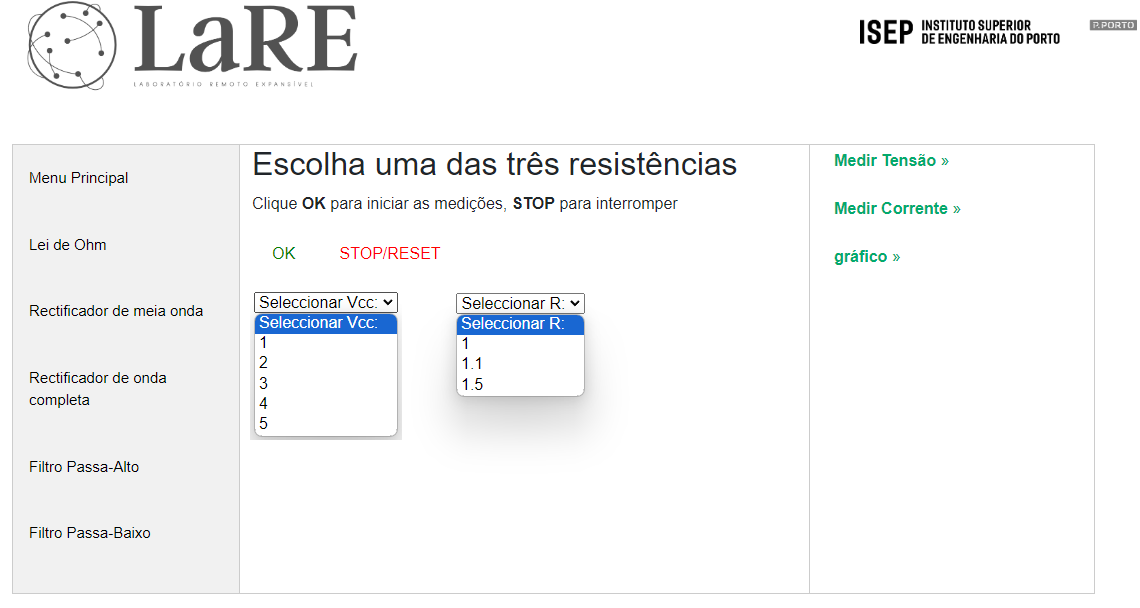
\includegraphics[width=1\textwidth]{figures/ohm_escolha.png}
    \caption{Experiência Lei de Ohm}
    \label{fig:pagohm}
\end{figure}

\begin{figure}[hbtp]
    \centering
    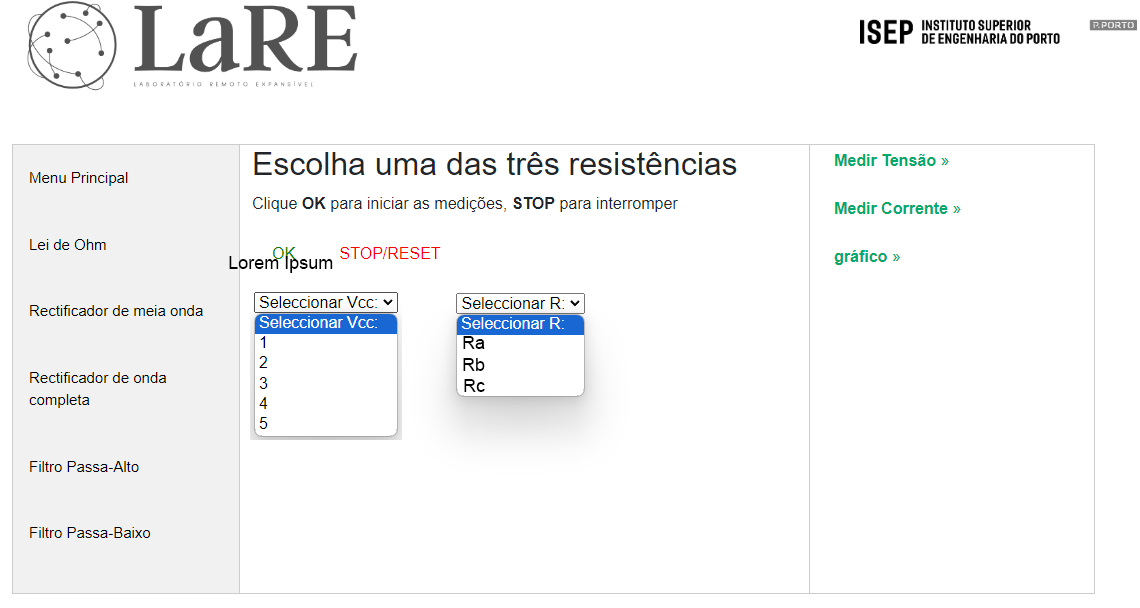
\includegraphics[width=1\textwidth]{figures/ohm_escolha_abc.png}
    \caption{Experiência Lei de Ohm - Resistências desconhecidas}
    \label{fig:pagohmabc}
\end{figure}

Na implementação desta experiência foram criados os ficheiros \textit{ohm.html}, como se pode ver, por exemplo, na Figura \ref{fig:pagohm} e o ficheiro \textit{configVB.py}

\subsection{Configuração do VirtualBench}
Da forma como está implementado o controlo da experiência, por parte do utilizador, levanta alguns pro

\section{qualquer merda que ainda não sei o quê}

Após análise e estudo da informação presente no \textit{site} do \textit{Flask} e nos tutoriais mencionados em cima, definiu-se e implementou-se a página de autenticação no ficheiro \textit{auth.py}, tal como pode ser visto na Figura \ref{fig:paglogin}:

\begin{figure}[hbtp]
    \centering
    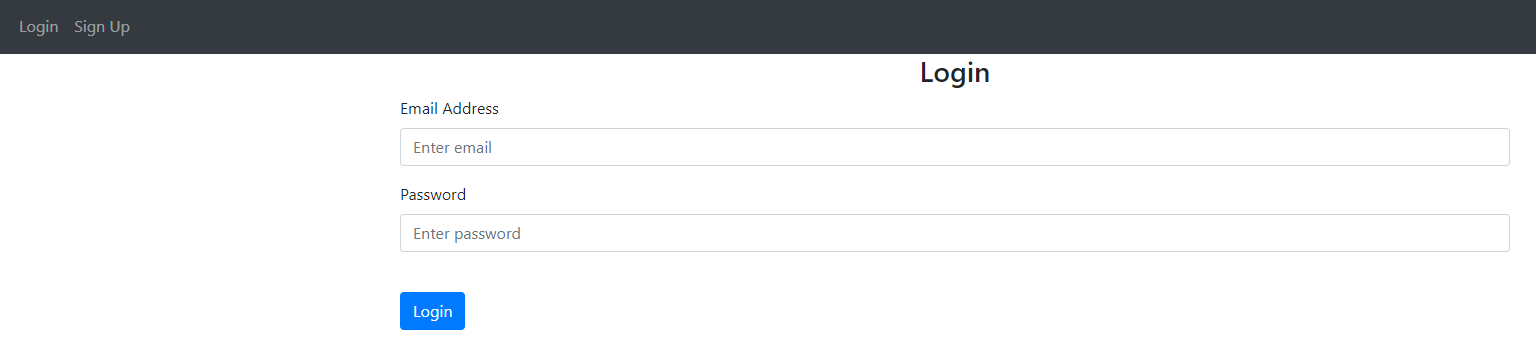
\includegraphics[width=1\textwidth]{figures/login.png}
    \caption{Página de \textit{login}}
    \label{fig:paglogin}
\end{figure}

Um exemplo de como foi implementada a função \textit{login}() está representada na Listagem \ref{lst:exemplologin} e a rota está definida para a página \textit{/login}, como apresentado na mesma Figura, linha 17.

Os dados de \textit{login} e registo são guardados na directoria \textit{instance}, ficheiro \textit{database.db}.

Além da rota definida para o \textit{login}, as outras rotas definidas no ficheiro \textit{auth.py} foram as \textit{sign-up} e \textit{logout}. A estrutura base da função \textit{login}, representada na Listagem \ref{lst:exemplologin}, é idêntica para as restantes, sendo que ``/\textit{login''} representa a rota especificada, dentro da função há o código especifico inerentes a cada função e o \textit{return render\_template} indica qual a página a ser renderizada. 

A juntar às páginas que compõem a estrutura base do \textit{site}, representadas na Figura \ref{fig:estruturapastas}, há ainda a juntar as páginas que permitem ao utilizador interagir com as experiências do \acrshort{lare}. Neste caso, serão cinco páginas, correspondentes aos 5 circuitos definidos na Secção \ref{sec:solucaoproposta}.

O menu de escolha foi retirado do \textit{site} \href{https://www.w3schools.com/howto/howto_js_vertical_tabs.asp}{\textit{w3schools}} e modificado de acordo com as necessidades do projecto, tal como pode ser visto na Figura \ref{fig:pagmenu}.

\begin{figure}[hbtp]
    \centering
    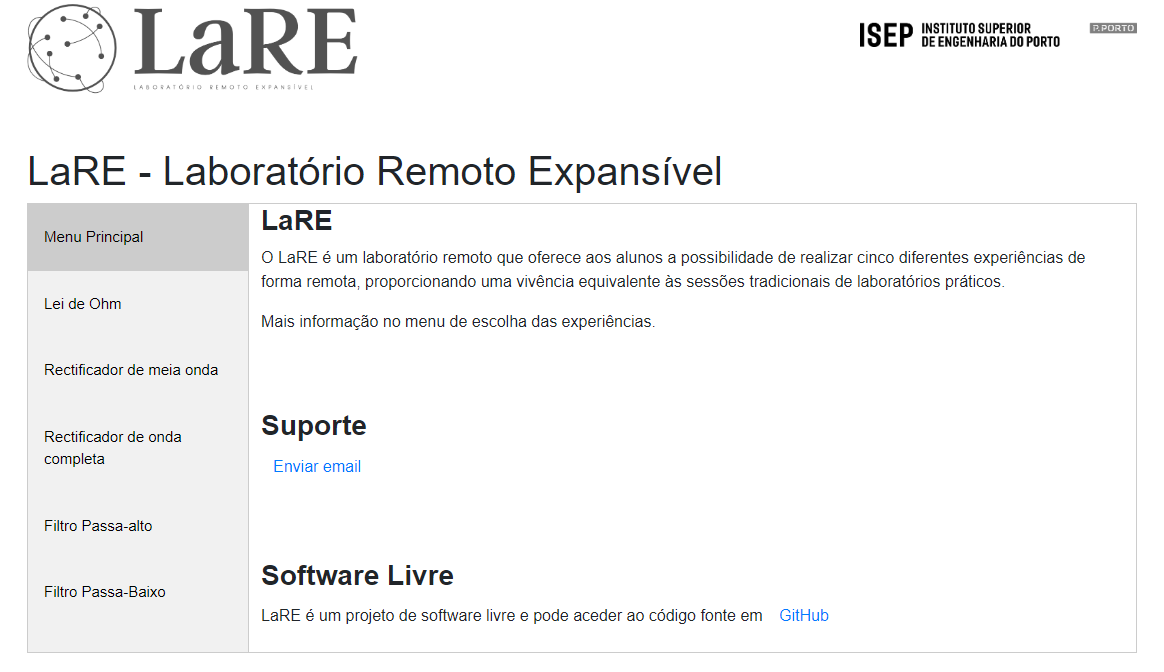
\includegraphics[width=1\textwidth]{figures/menupage.png}
    \caption{Página de menus}
    \label{fig:pagmenu}
\end{figure}

As páginas referentes às experiências seguem a mesma estrutura de menus.

\sout{Uma das partes mais cruciais e que levantou mais dificuldades foi a comunicação e o envio de parâmetros entre as páginas \acrshort{html} e o \textit{Flask}.}